% !TEX root = ../../main.tex


\begin{figure}[p]
{\scriptsize \texthv{\textbf{(a)} Before genotype error}} \\
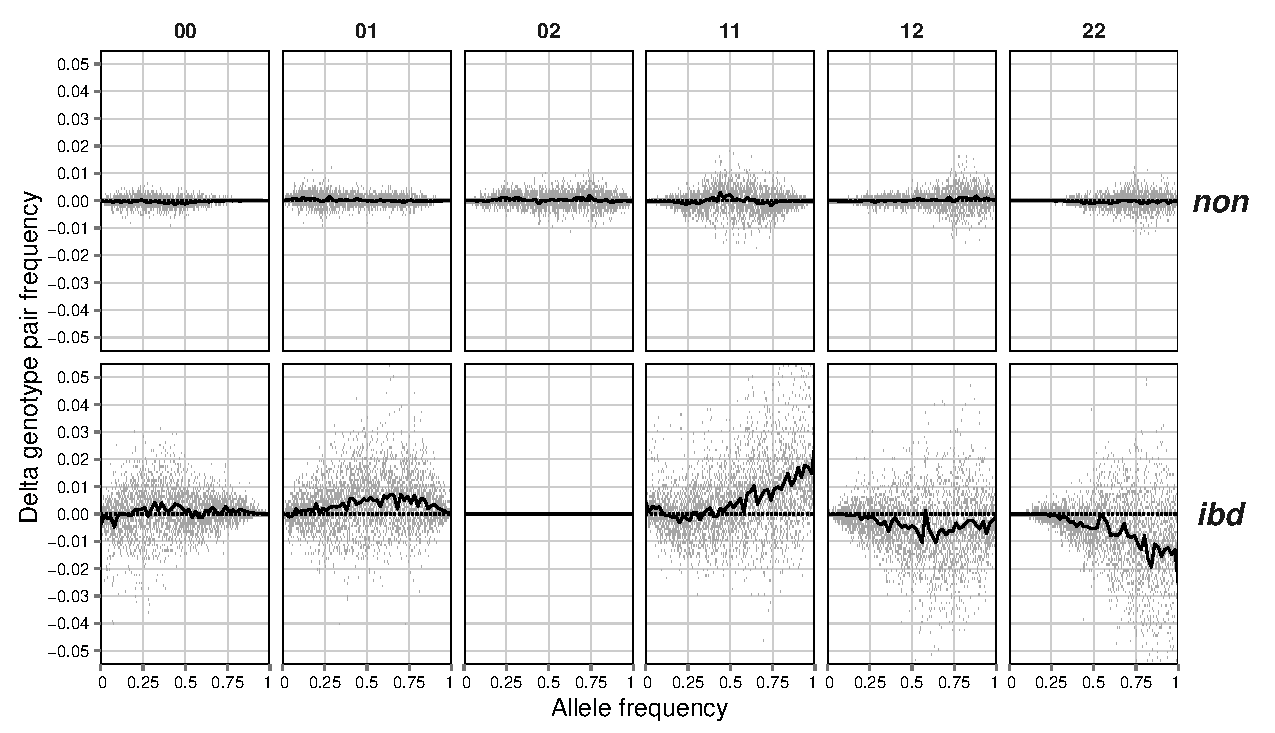
\includegraphics[width=\textwidth]{./img/ch4/hmm_emission_delta_tru}
{\scriptsize \texthv{\textbf{(b)} After genotype error}} \\
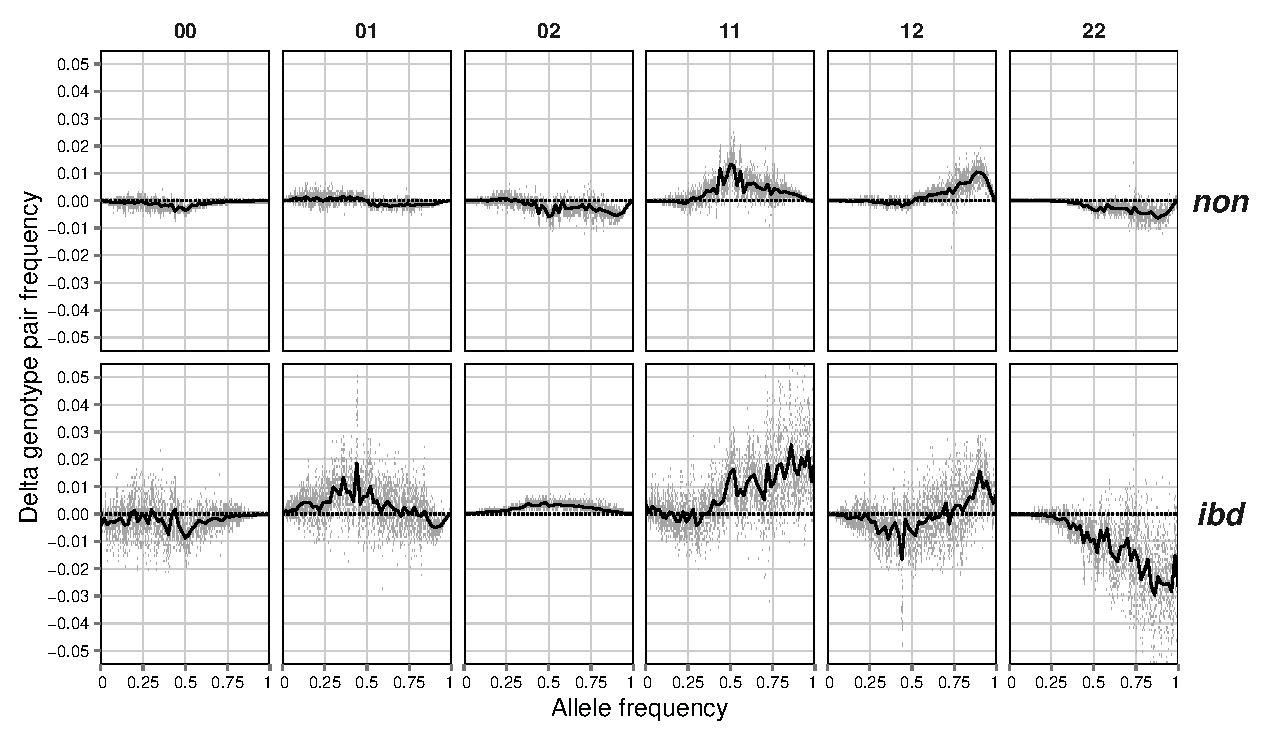
\includegraphics[width=\textwidth]{./img/ch4/hmm_emission_delta_err}
\Caption{Difference between empirical and expected proportions of genotype pairs}
{In total, \n{500000} segments were sampled in \emph{non} and \emph{ibd} as determined from coalescent records.
Segments were aggregated by allele frequency to calculate empirical proportions for each of the \n{6} possible genotype pairs (${g_{k_1,k_2}}$, indicated above each panel).
Delta values were calculated by subtracting empirical from expected proportions; the latter were calculated using \cref{eq:genpairnon,eq:genpairibd} under \emph{non} and \emph{ibd}, respectively.
Each panel is a scatterplot showing the deviation at each discrete step in allele frequency.
The mean (${\pm\text{SE}}$) of delta values was calculated in steps of 1\% allele frequency; indicated by the \emph{black} line.
Results in Panel~\textbf{(a)} were generated on data before the inclusion of genotype error, $D$, and Panel~\textbf{(b)} on data after genotype error was included, $D^{\ast}$.}
{fig:hmm_emission_delta}
\end{figure}
